\documentclass[a4paper,oneside,14pt]{extreport}

\usepackage[T2A]{fontenc}
\usepackage[utf8]{inputenc}
\usepackage[english,russian]{babel}

%\usepackage[left=30mm, right=20mm, top=20mm, bottom=20mm]{geometry}
\usepackage[left=20mm, right=10mm, top=5mm, bottom=20mm]{geometry}

\usepackage{microtype}
\sloppy

\usepackage{setspace}
\onehalfspacing

\usepackage{indentfirst}
\setlength{\parindent}{12.5mm}

\usepackage{titlesec}
\titleformat{\chapter}{\LARGE\bfseries}{\thechapter}{14pt}{\LARGE\bfseries}
\titlespacing*{\chapter}{\parindent}{0mm}{5mm}
\titleformat{\section}{\Large\bfseries}{\thesection}{14pt}{\Large\bfseries}

\addto{\captionsrussian}{\renewcommand*{\contentsname}{Содержание}}
\usepackage{natbib}
\renewcommand{\bibsection}{\chapter*{Список использованных источников}}

\usepackage{caption}

\usepackage{wrapfig}
\usepackage{float}

\usepackage{graphicx}
\newcommand{\imgwc}[4]
{
	\begin{figure}[#1]
		\center{\includegraphics[width=#2]{inc/img/#3}}
		\caption{#4}
		\label{img:#3}
	\end{figure}
}
\newcommand{\imghc}[4]
{
	\begin{figure}[#1]
		\center{\includegraphics[height=#2]{inc/img/#3}}
		\caption{#4}
		\label{img:#3}
	\end{figure}
}
\newcommand{\imgsc}[4]
{
	\begin{figure}[#1]
		\center{\includegraphics[scale=#2]{inc/img/#3}}
		\caption{#4}
		\label{img:#3}
	\end{figure}
}

\usepackage{pgfplots}
\pgfplotsset{compat=newest}

\usepackage{listings}
\usepackage{listingsutf8}
\lstset{
	basicstyle=\footnotesize\ttfamily,
	keywordstyle=\color{blue},
	stringstyle=\color{red},
	commentstyle=\color{gray},
	numbers=left,
	numberstyle=\tiny,
	numbersep=5pt,
	frame=false,
	breaklines=true,
	breakatwhitespace=true,
	inputencoding=utf8/koi8-r
}

\lstdefinestyle{c}{
	language=C++,
	backgroundcolor=\color{white},
	basicstyle=\footnotesize\ttfamily,
	keywordstyle=\color{blue},
	stringstyle=\color{red},
	commentstyle=\color{gray},
	directivestyle=\color{orange},
	numbers=left,
	numberstyle=\tiny,
	stepnumber=1,
	numbersep=5pt,
	frame=single,
	tabsize=4,
	captionpos=t,
	breaklines=true,
	breakatwhitespace=true,
	escapeinside={\#*}{*)},
	morecomment=[l][\color{magenta}]{\#},
	columns=fullflexible
}

\newcommand{\code}[1]{\texttt{#1}}

\usepackage{amsmath}
\usepackage{amssymb}

\usepackage[unicode]{hyperref}
\hypersetup{hidelinks}

\makeatletter
\newcommand{\vhrulefill}[1]
{
	\leavevmode\leaders\hrule\@height#1\hfill \kern\z@
}
\makeatother

\begin{document}

\begin{titlepage}
	\centering
	
	\vspace{-2.2mm}
	\vhrulefill{0.9mm}\\
	\vspace{-7mm}
	\vhrulefill{0.2mm}\\
	\vspace{2mm}
	
	\vspace{50mm}
	
	\vspace{30mm}
	
	\textbf{Отчет по лабораторной работе №7}\\
	По курсу: <<Фильтрация и прогнозирование данных>>\\
	Тема: <<Решение обратной задачи>>\\
	
	\vspace{60mm}
	
	\hspace{70mm} Студент:       \hfill Пронин~А.~С.\\
	\hspace{70mm} Группа:        \hfill МСМТ231\\
	\hspace{70mm} Преподаватель: \hfill Зотов~Л.~В.\\
	%	\hspace{70mm} Оценка:        \hfill \hrulefill\\
	
	\vfill
	
	Москва\\
	\the\year
\end{titlepage}

\setcounter{page}{2}

\chapter*{Лабораторная работа 7}

%\textbf{Задание 1}

Для выполнения ЛР7 необходимо использовать выходной сигнал из ЛР6, поэтому сначала запишем его в файл, а затем считаем из новой программы и добавим незначительный шум (рис. \ref{task1_mn}-\ref{task1_mn2}):

\begin{figure}[!h]
	\center{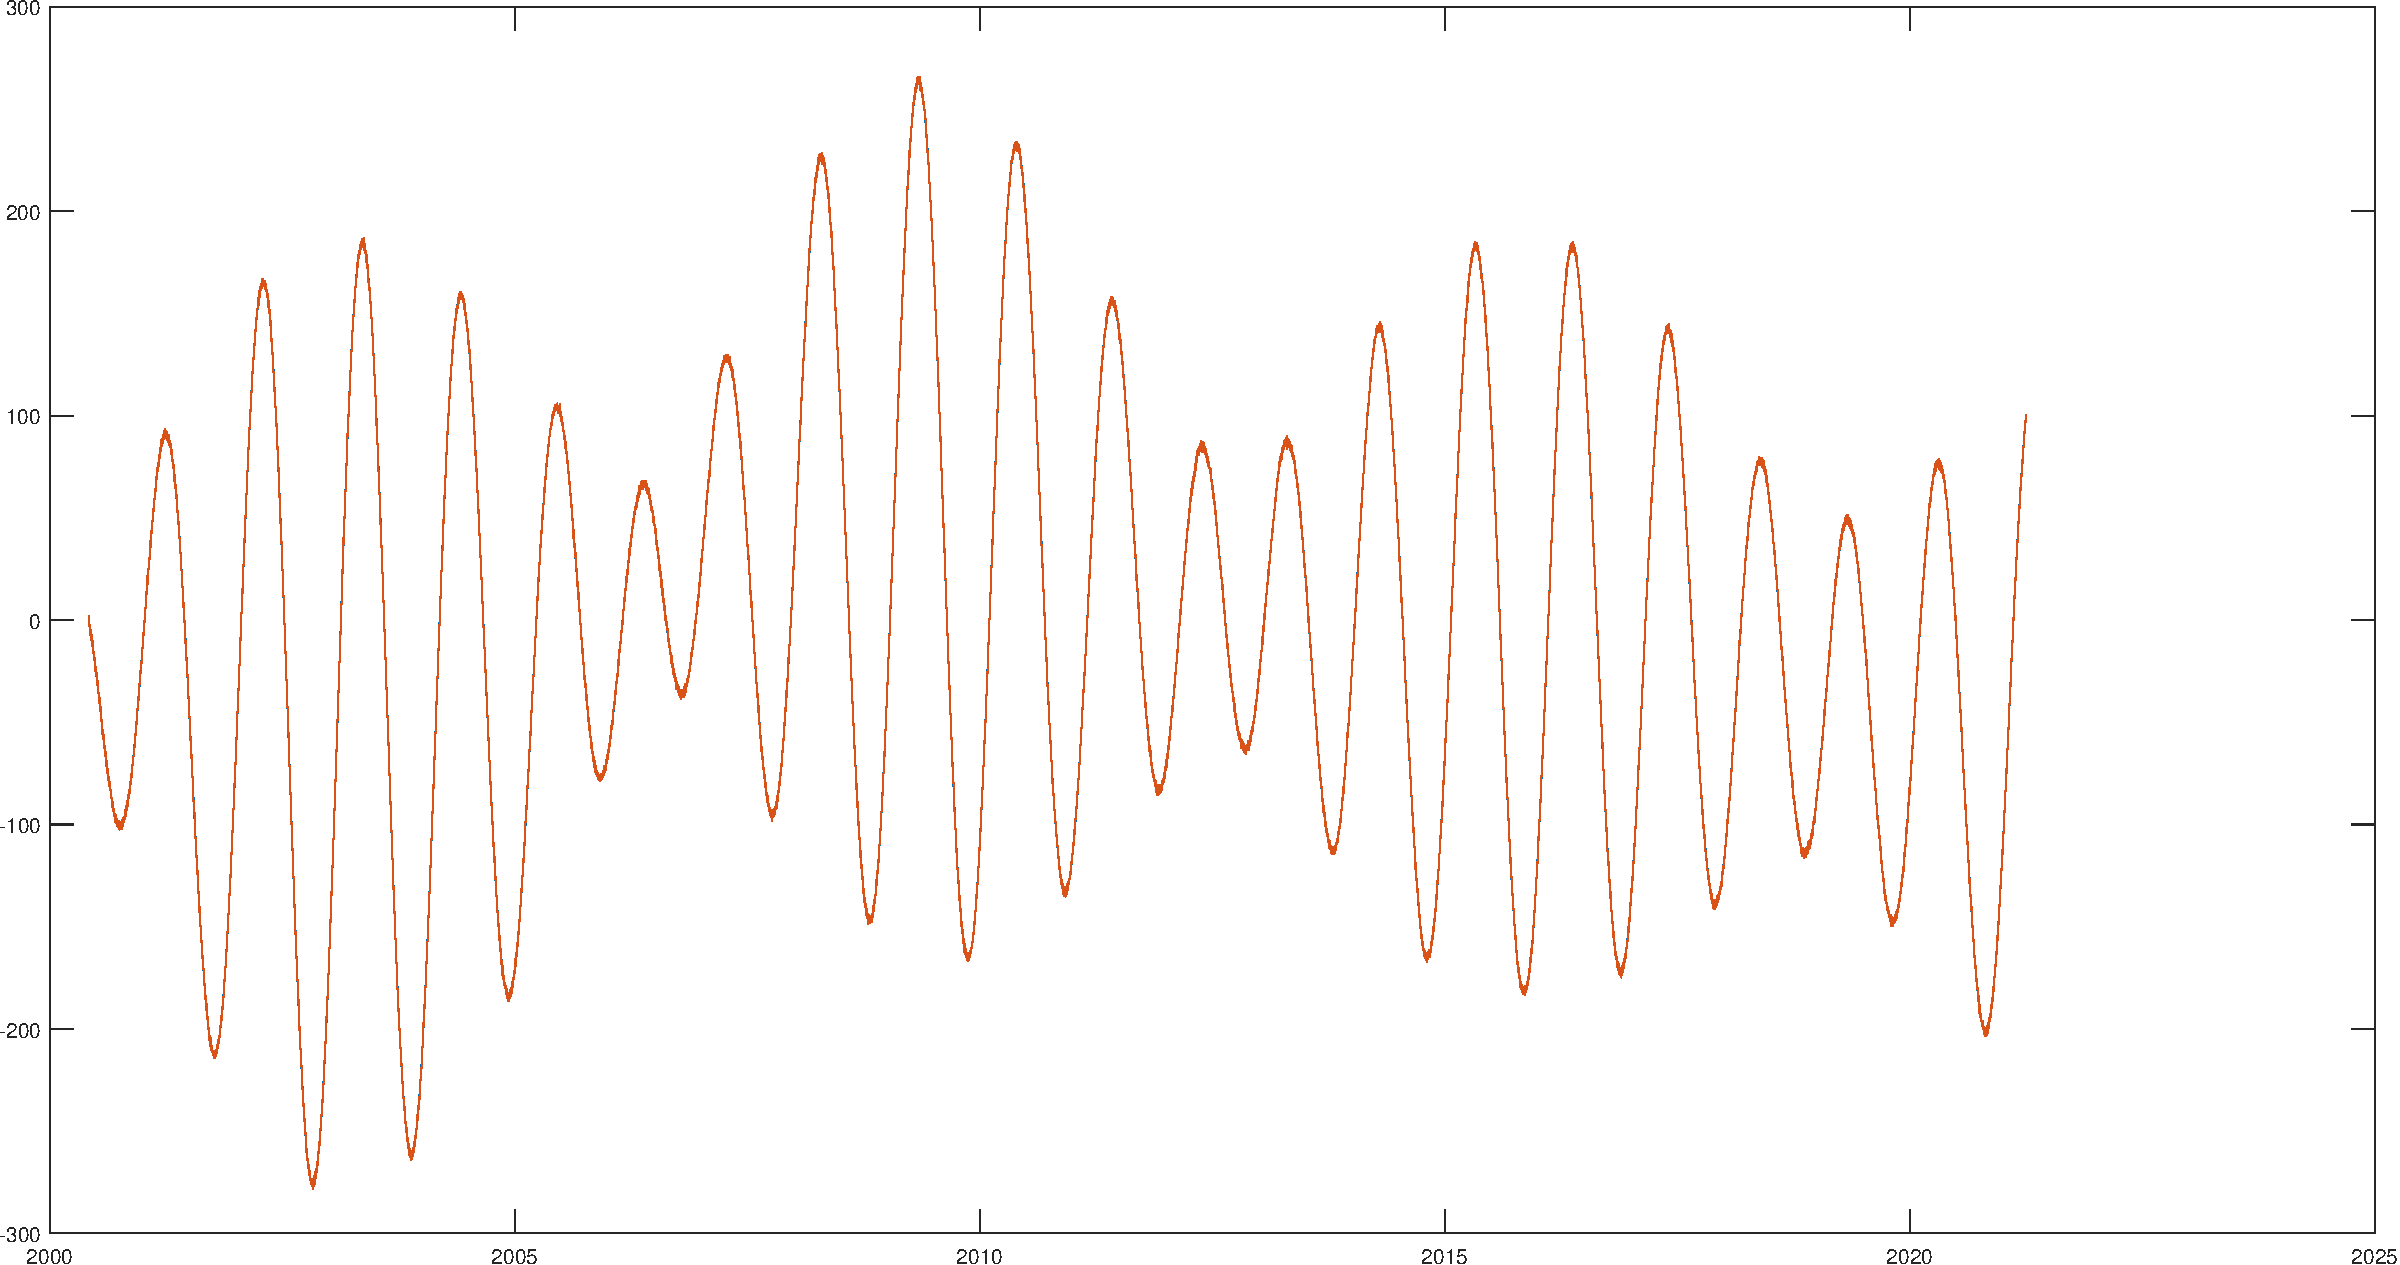
\includegraphics[width=0.9\linewidth]{inc/task1_mn}}
	\caption{Первые 30000 точек выходного сигнала из ЛР6 с незначительным шумом}
	\label{task1_mn}
\end{figure}

\begin{figure}[!h]
\center{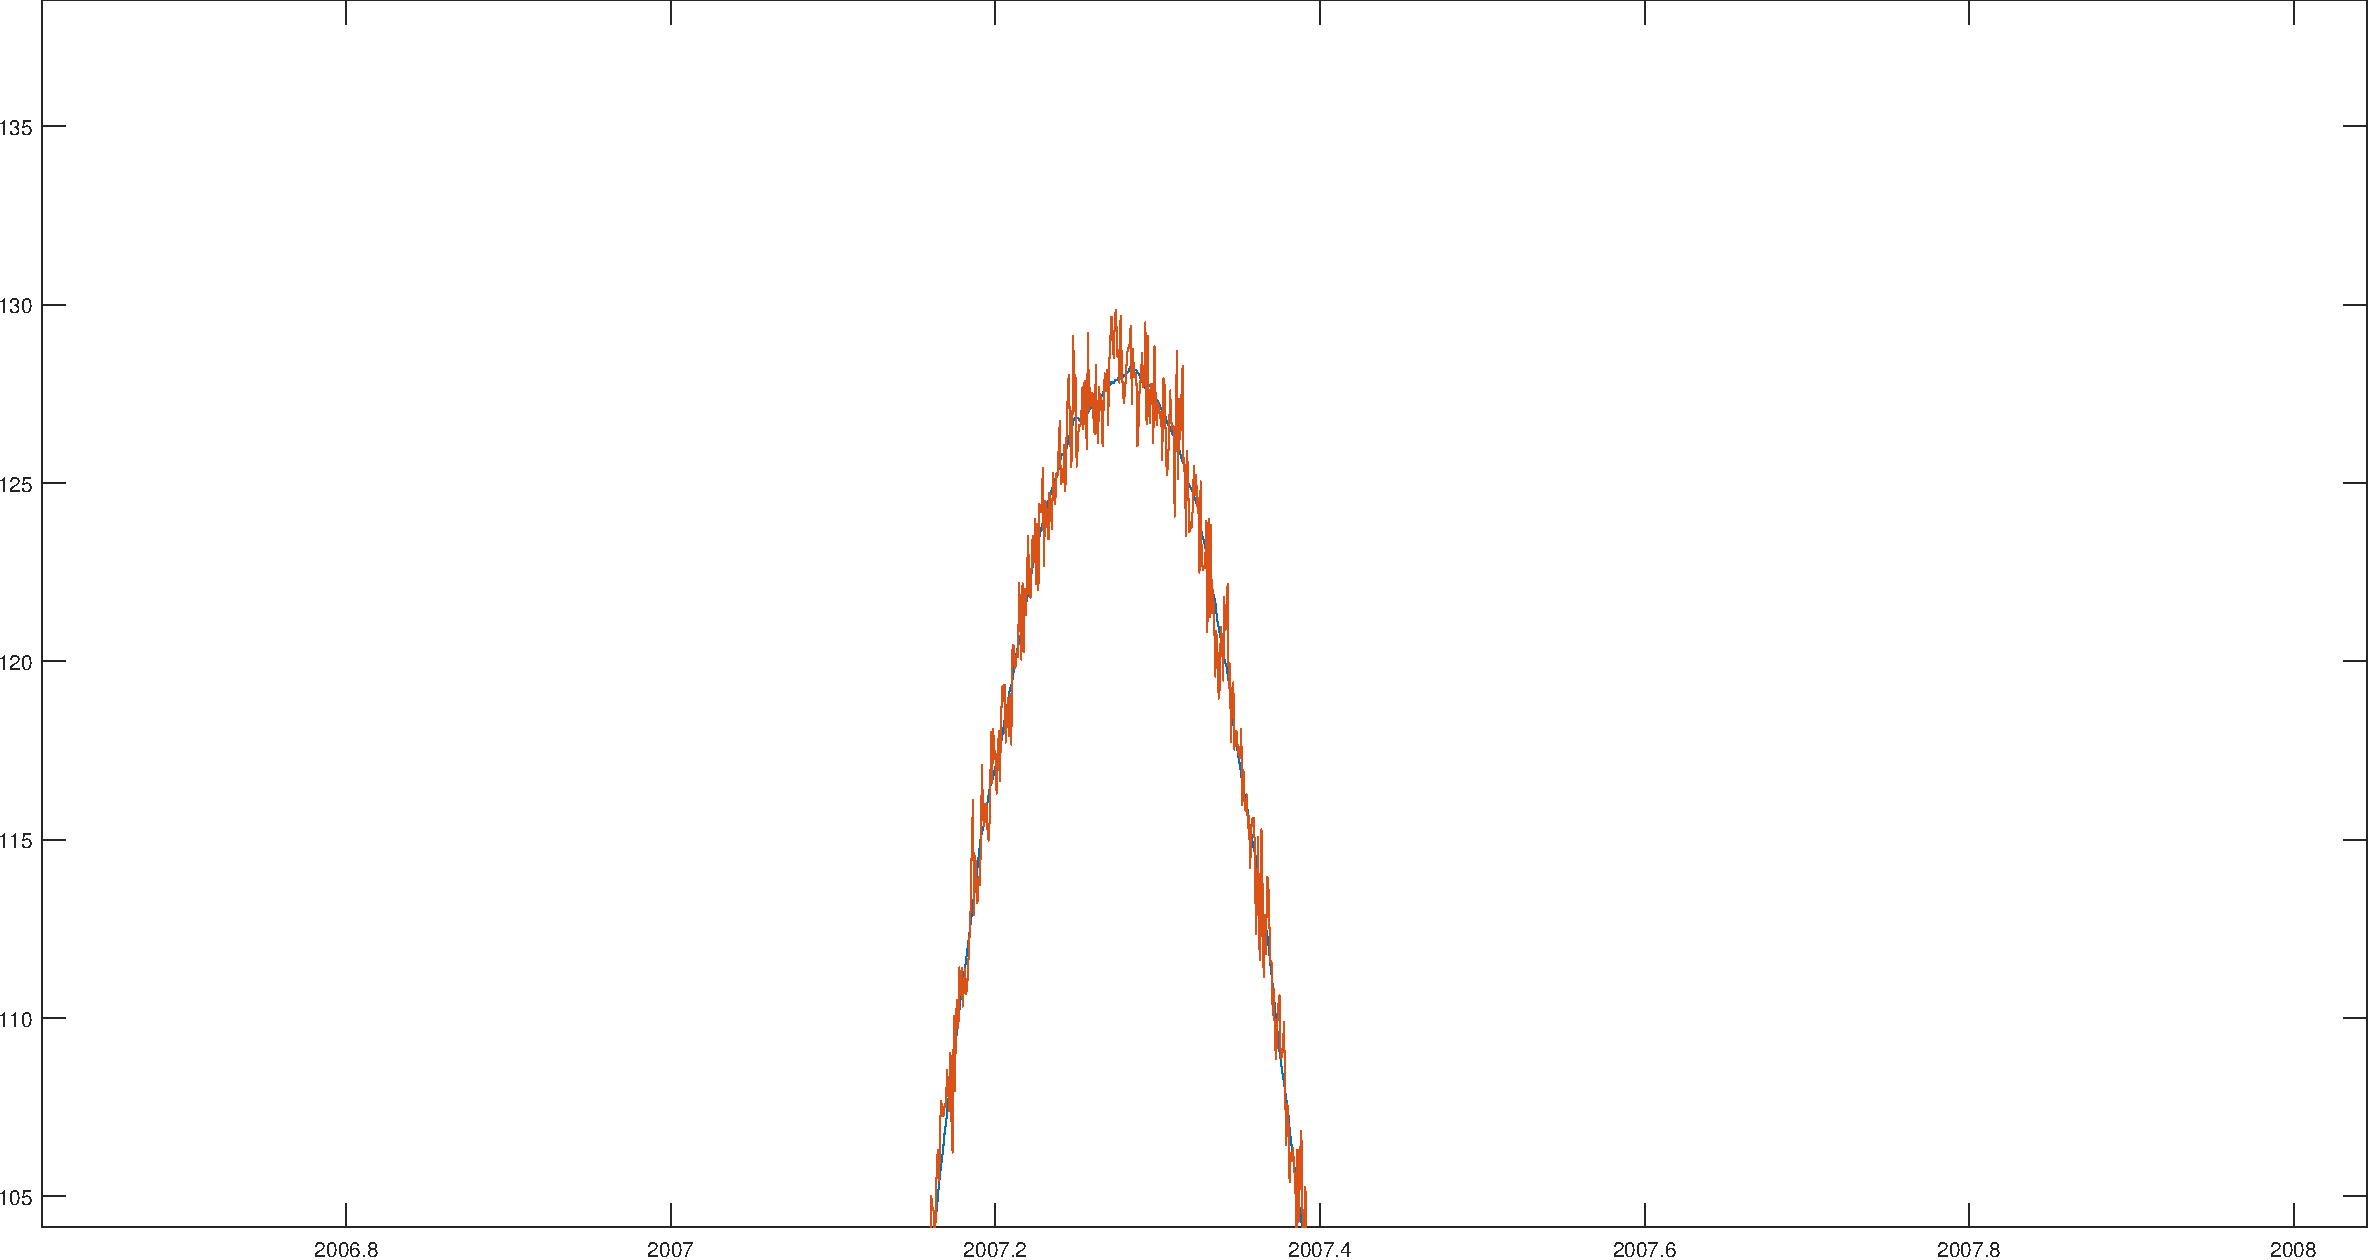
\includegraphics[width=0.9\linewidth]{inc/task1_mn2}}
\caption{Незначительный шум поверх выходного сигнала из ЛР6}
\label{task1_mn2}
\end{figure}

\newpage
Выведем для него спектр и вейвлет-скейлограмму (рис. \ref{task1_spectr1}-\ref{task1_cwt1}):

\begin{figure}[!h]
	\center{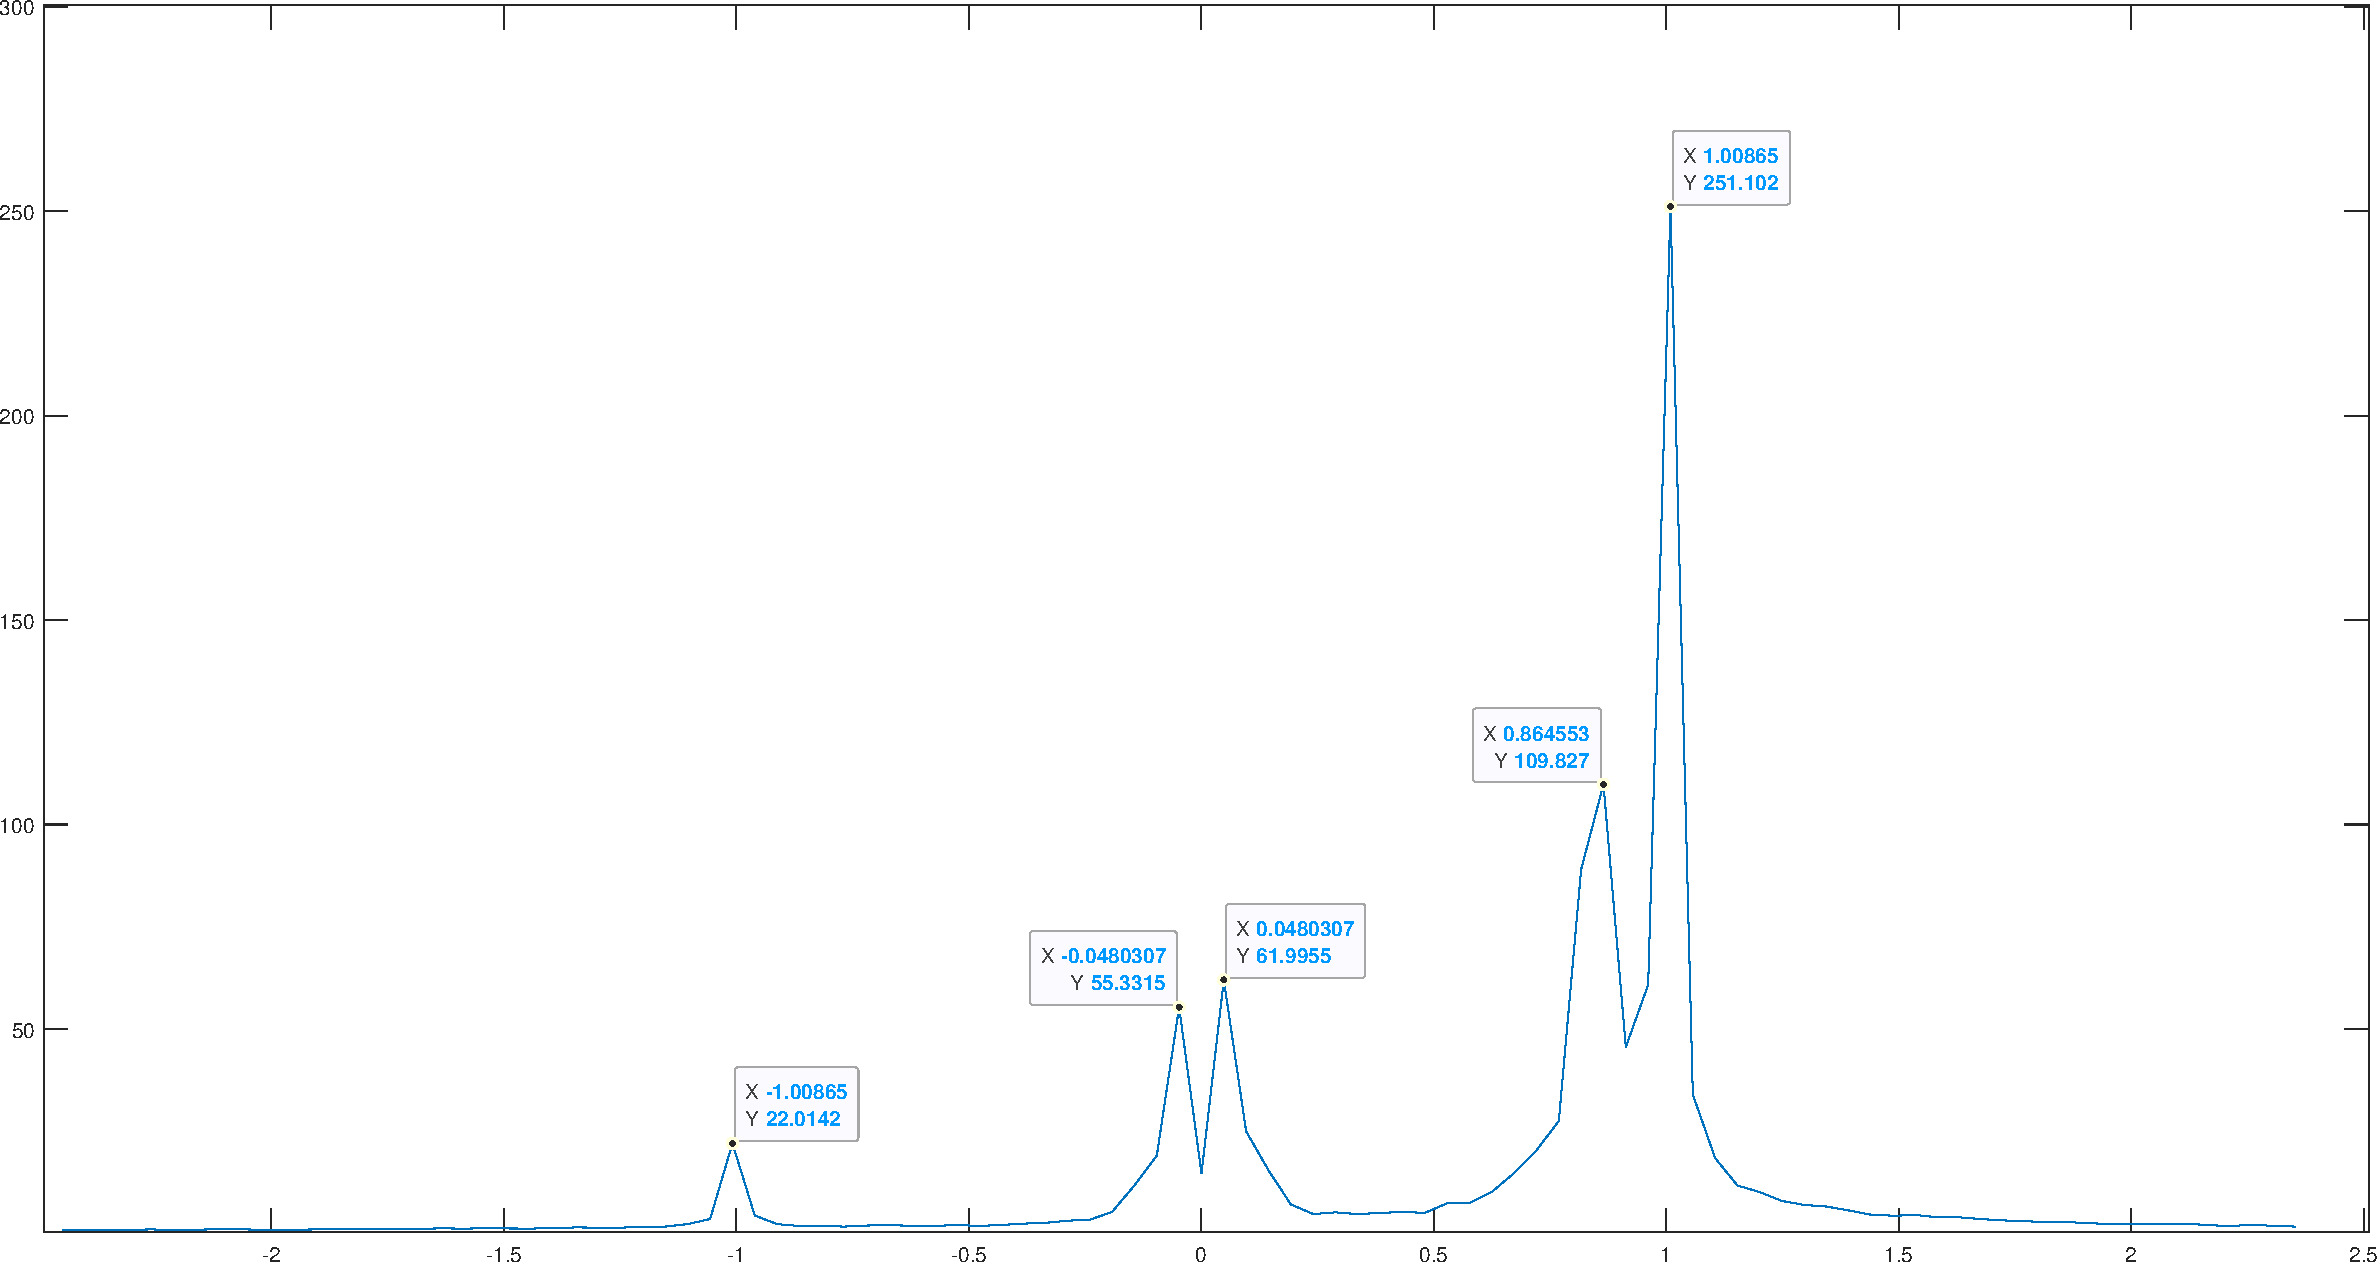
\includegraphics[width=1\linewidth]{inc/task1_spectr1}}
	\caption{Спектральная плотность мощности 1}
	\label{task1_spectr1}
\end{figure}

\begin{figure}[!h]
	\center{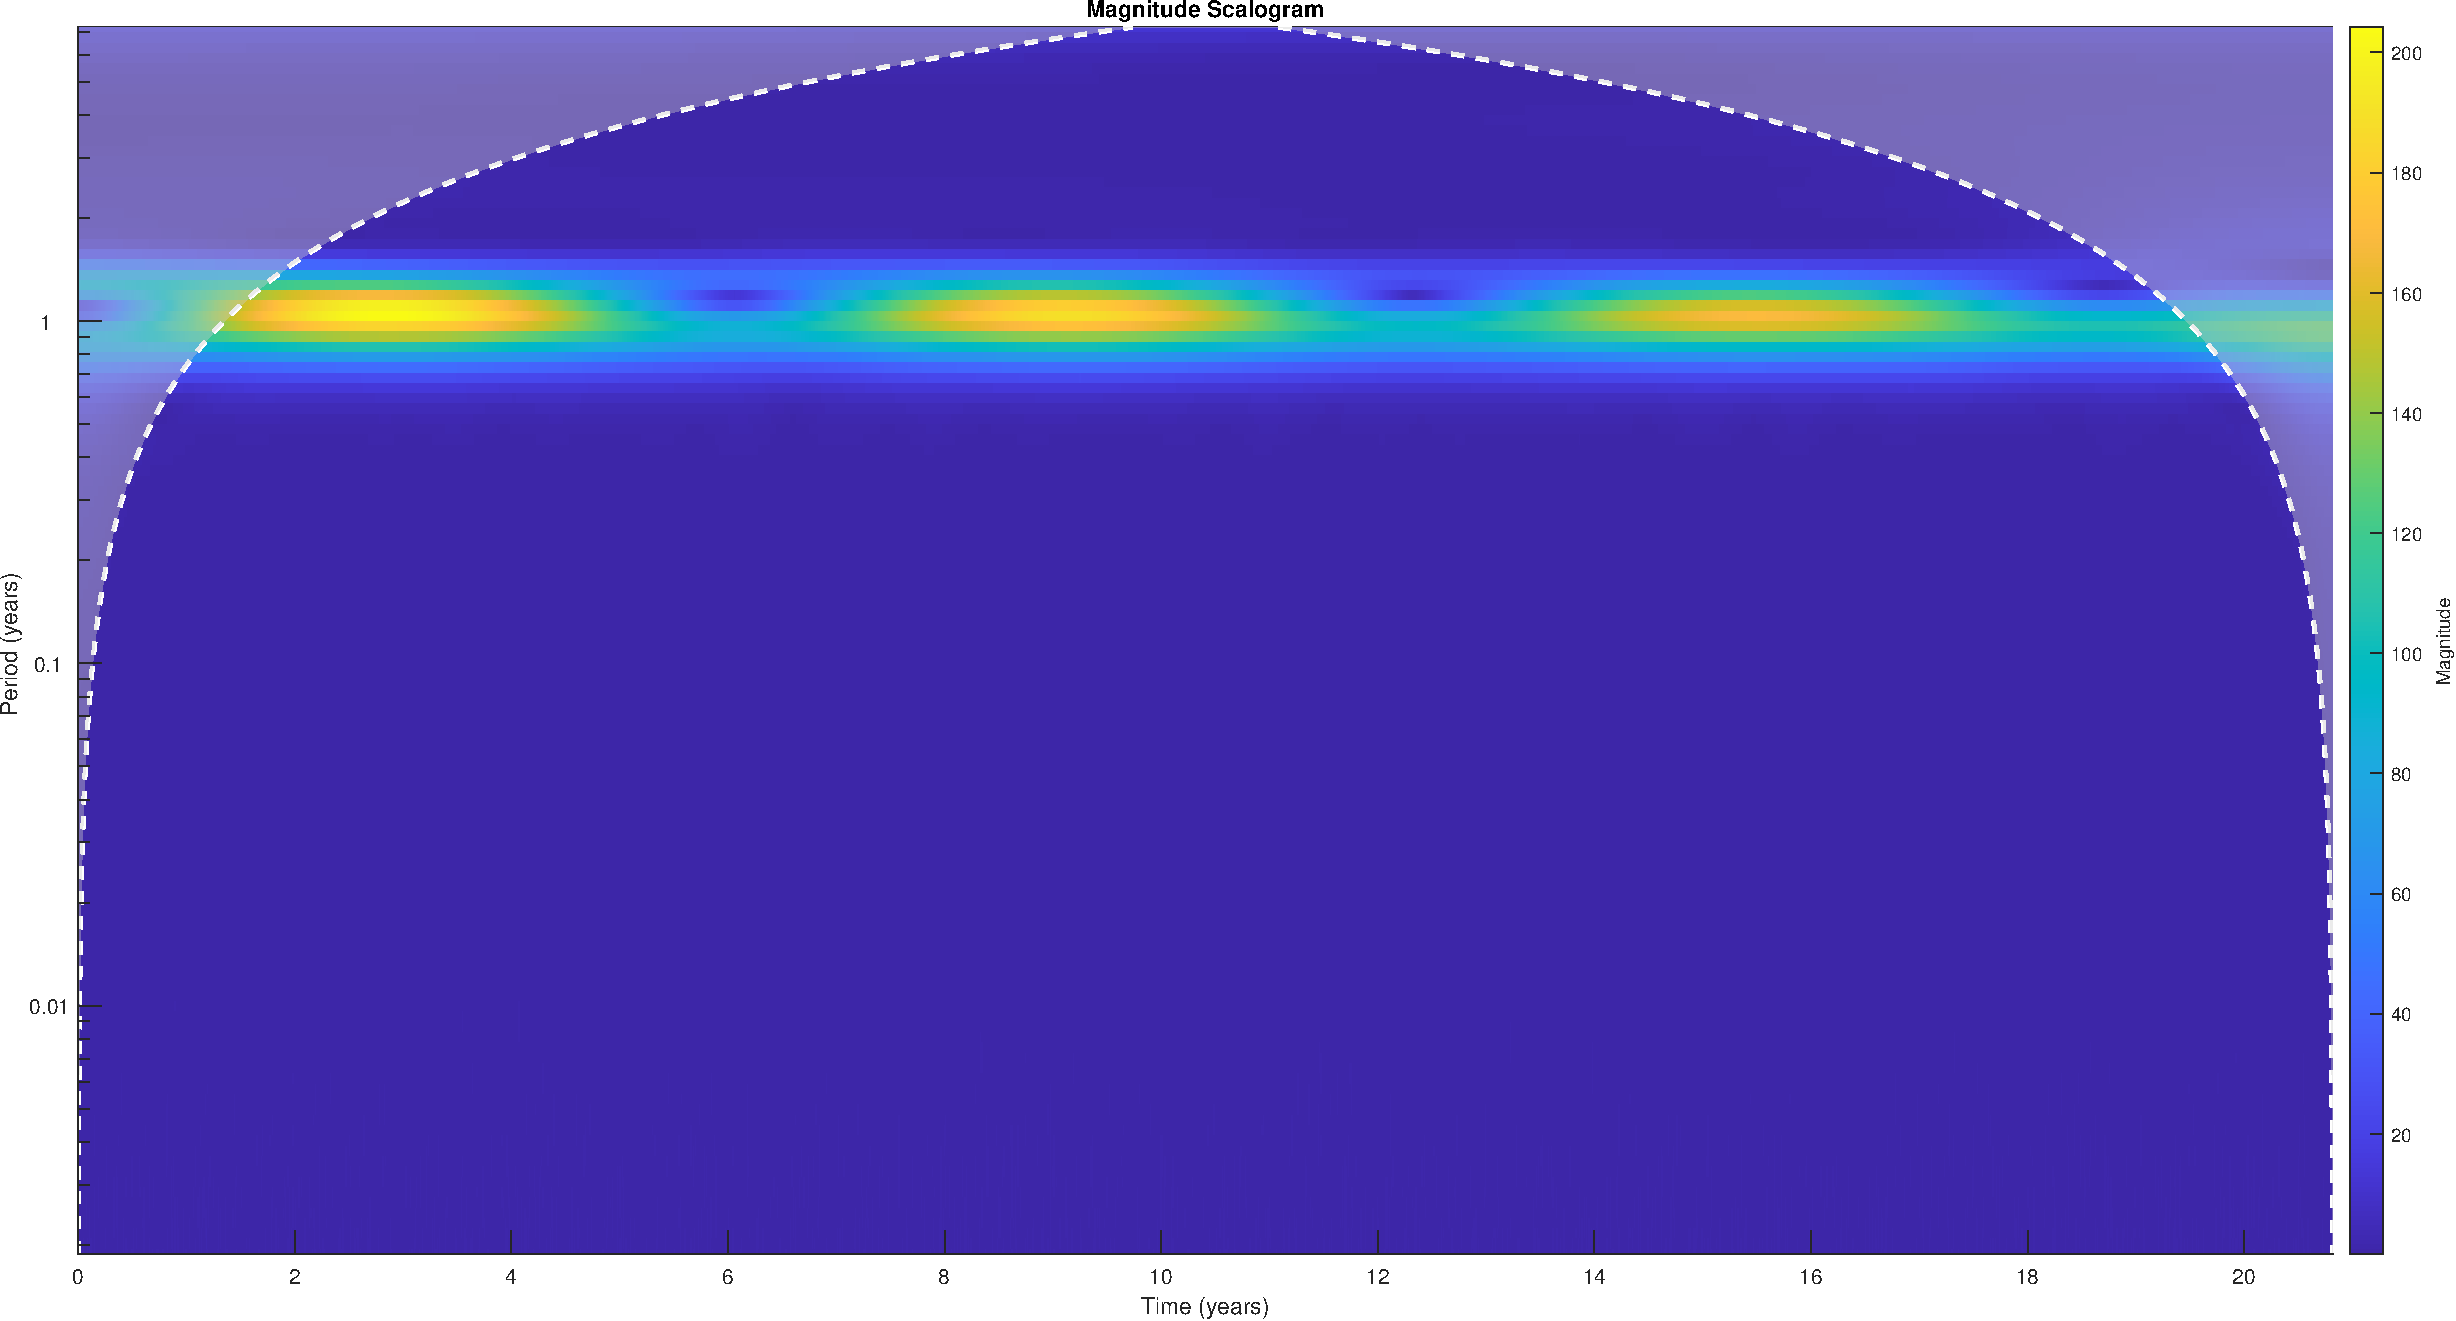
\includegraphics[width=1\linewidth]{inc/task1_cwt1}}
	\caption{Вейвлет-скейлограмма 1}
	\label{task1_cwt1}
\end{figure}

Как видно по графикам \ref{task1_spectr1}-\ref{task1_cwt1}, 30000 точек недостаточно чтобы уловить 8.86-летний и 18.6-летний циклы - они слились в один пик на СПМ, а на вейвлет-скейлограмме вовсе не отобразились. Поэтому попробуем взять все данные из файла за 90 лет и заново построить спектр и вейвлет-скейлограмму (рис. \ref{task1_spectr2}-\ref{task1_cwt2}):

\newpage
\begin{figure}[!h]
	\center{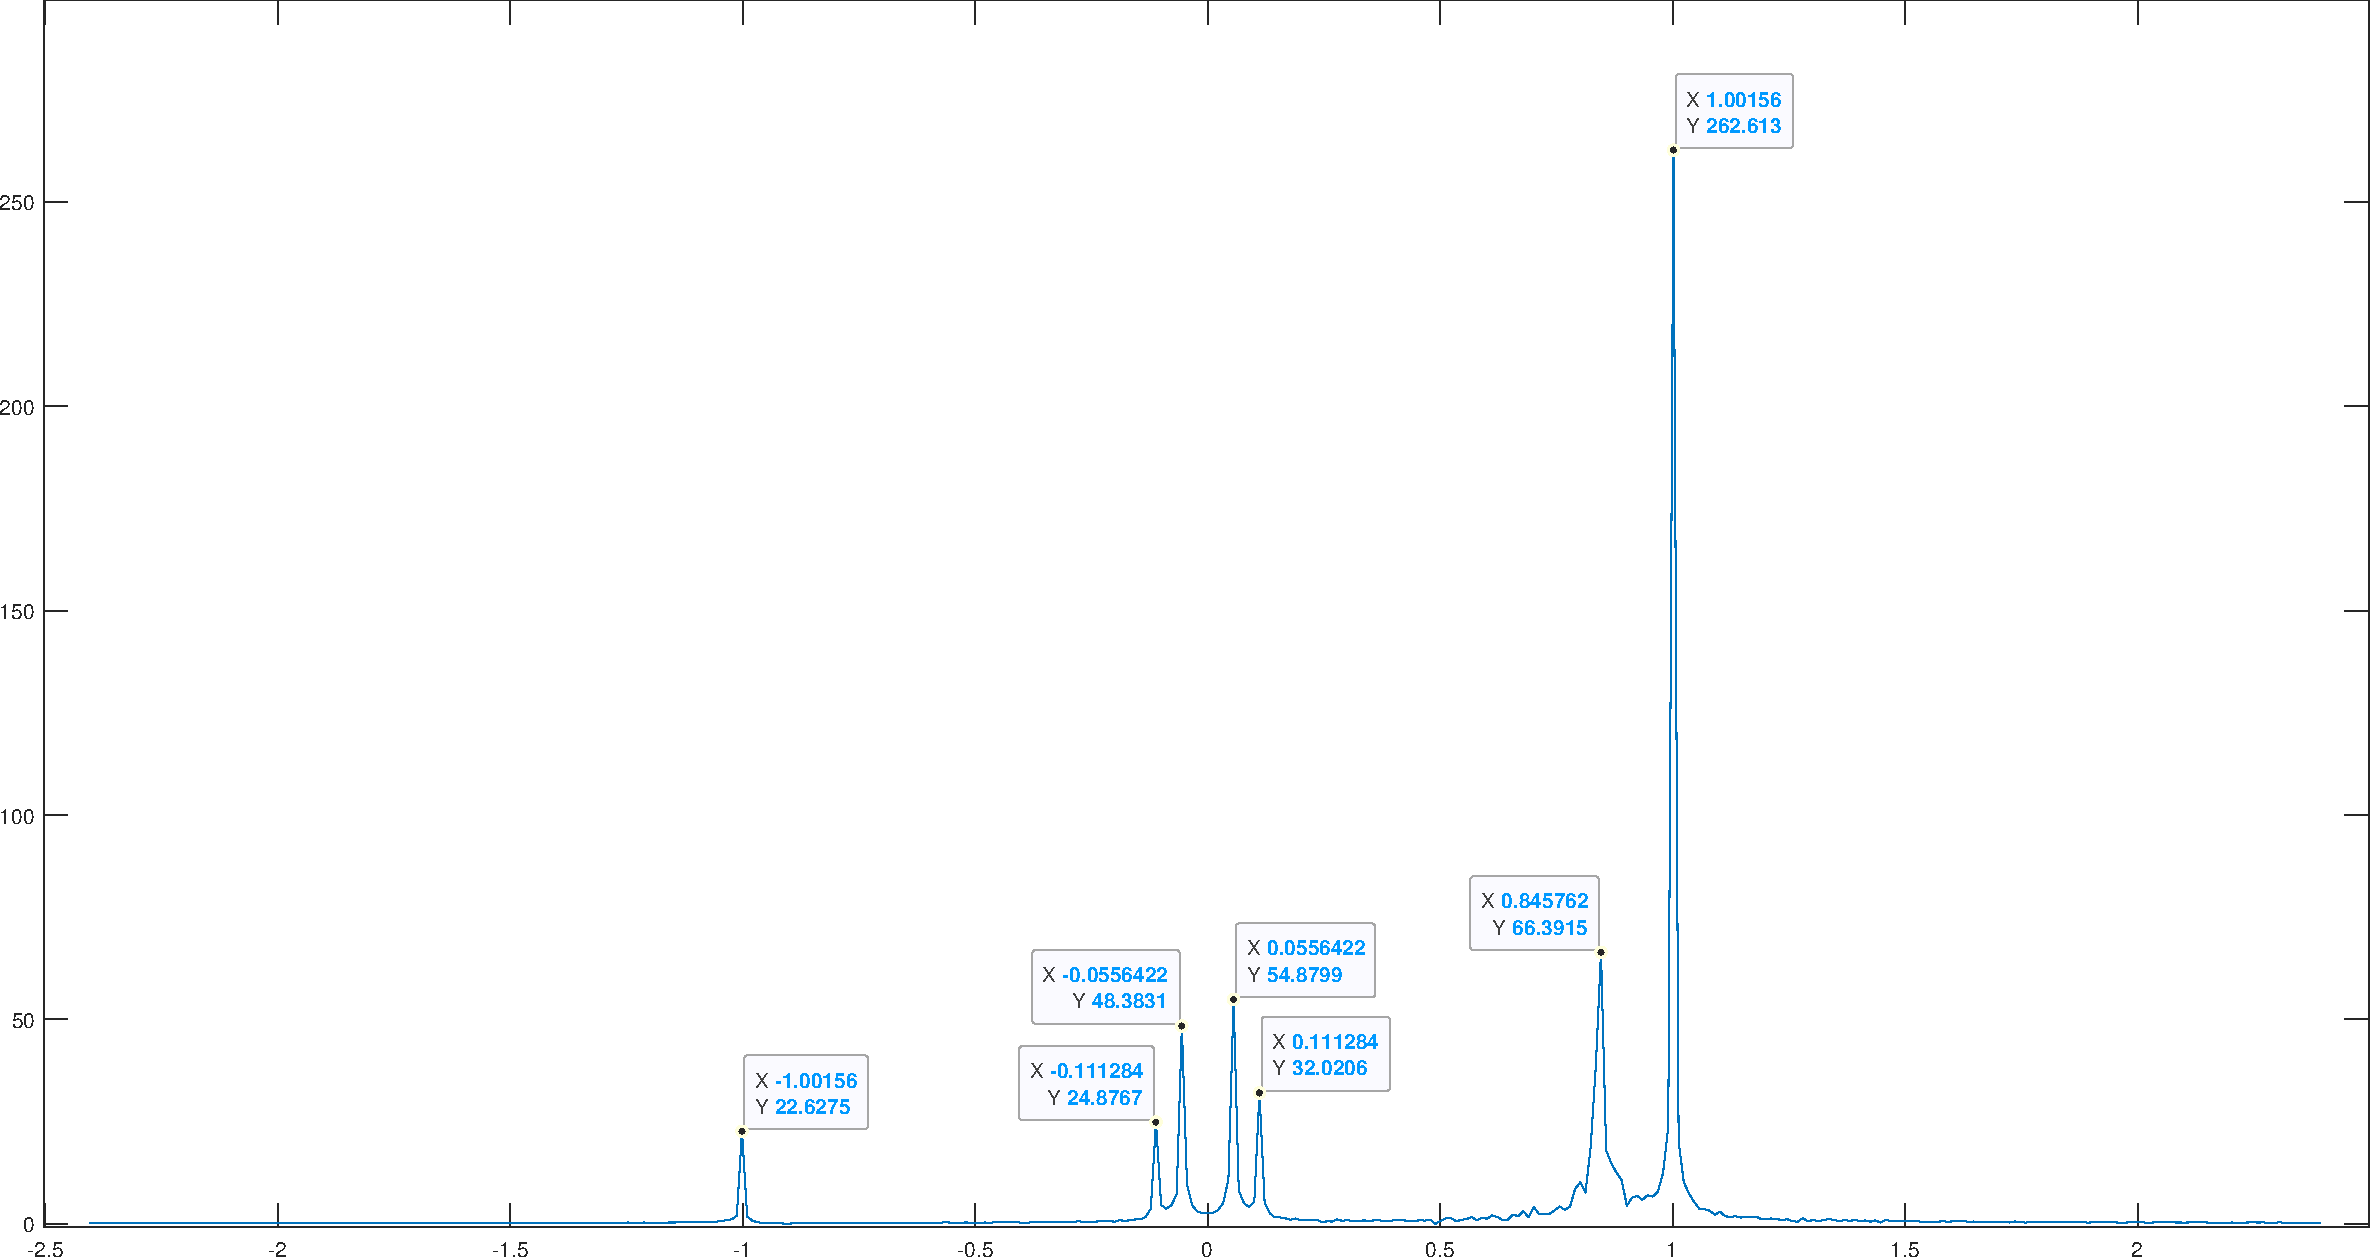
\includegraphics[width=1\linewidth]{inc/task1_spectr2}}
	\caption{Спектральная плотность мощности 2}
	\label{task1_spectr2}
\end{figure}

\begin{figure}[!h]
	\center{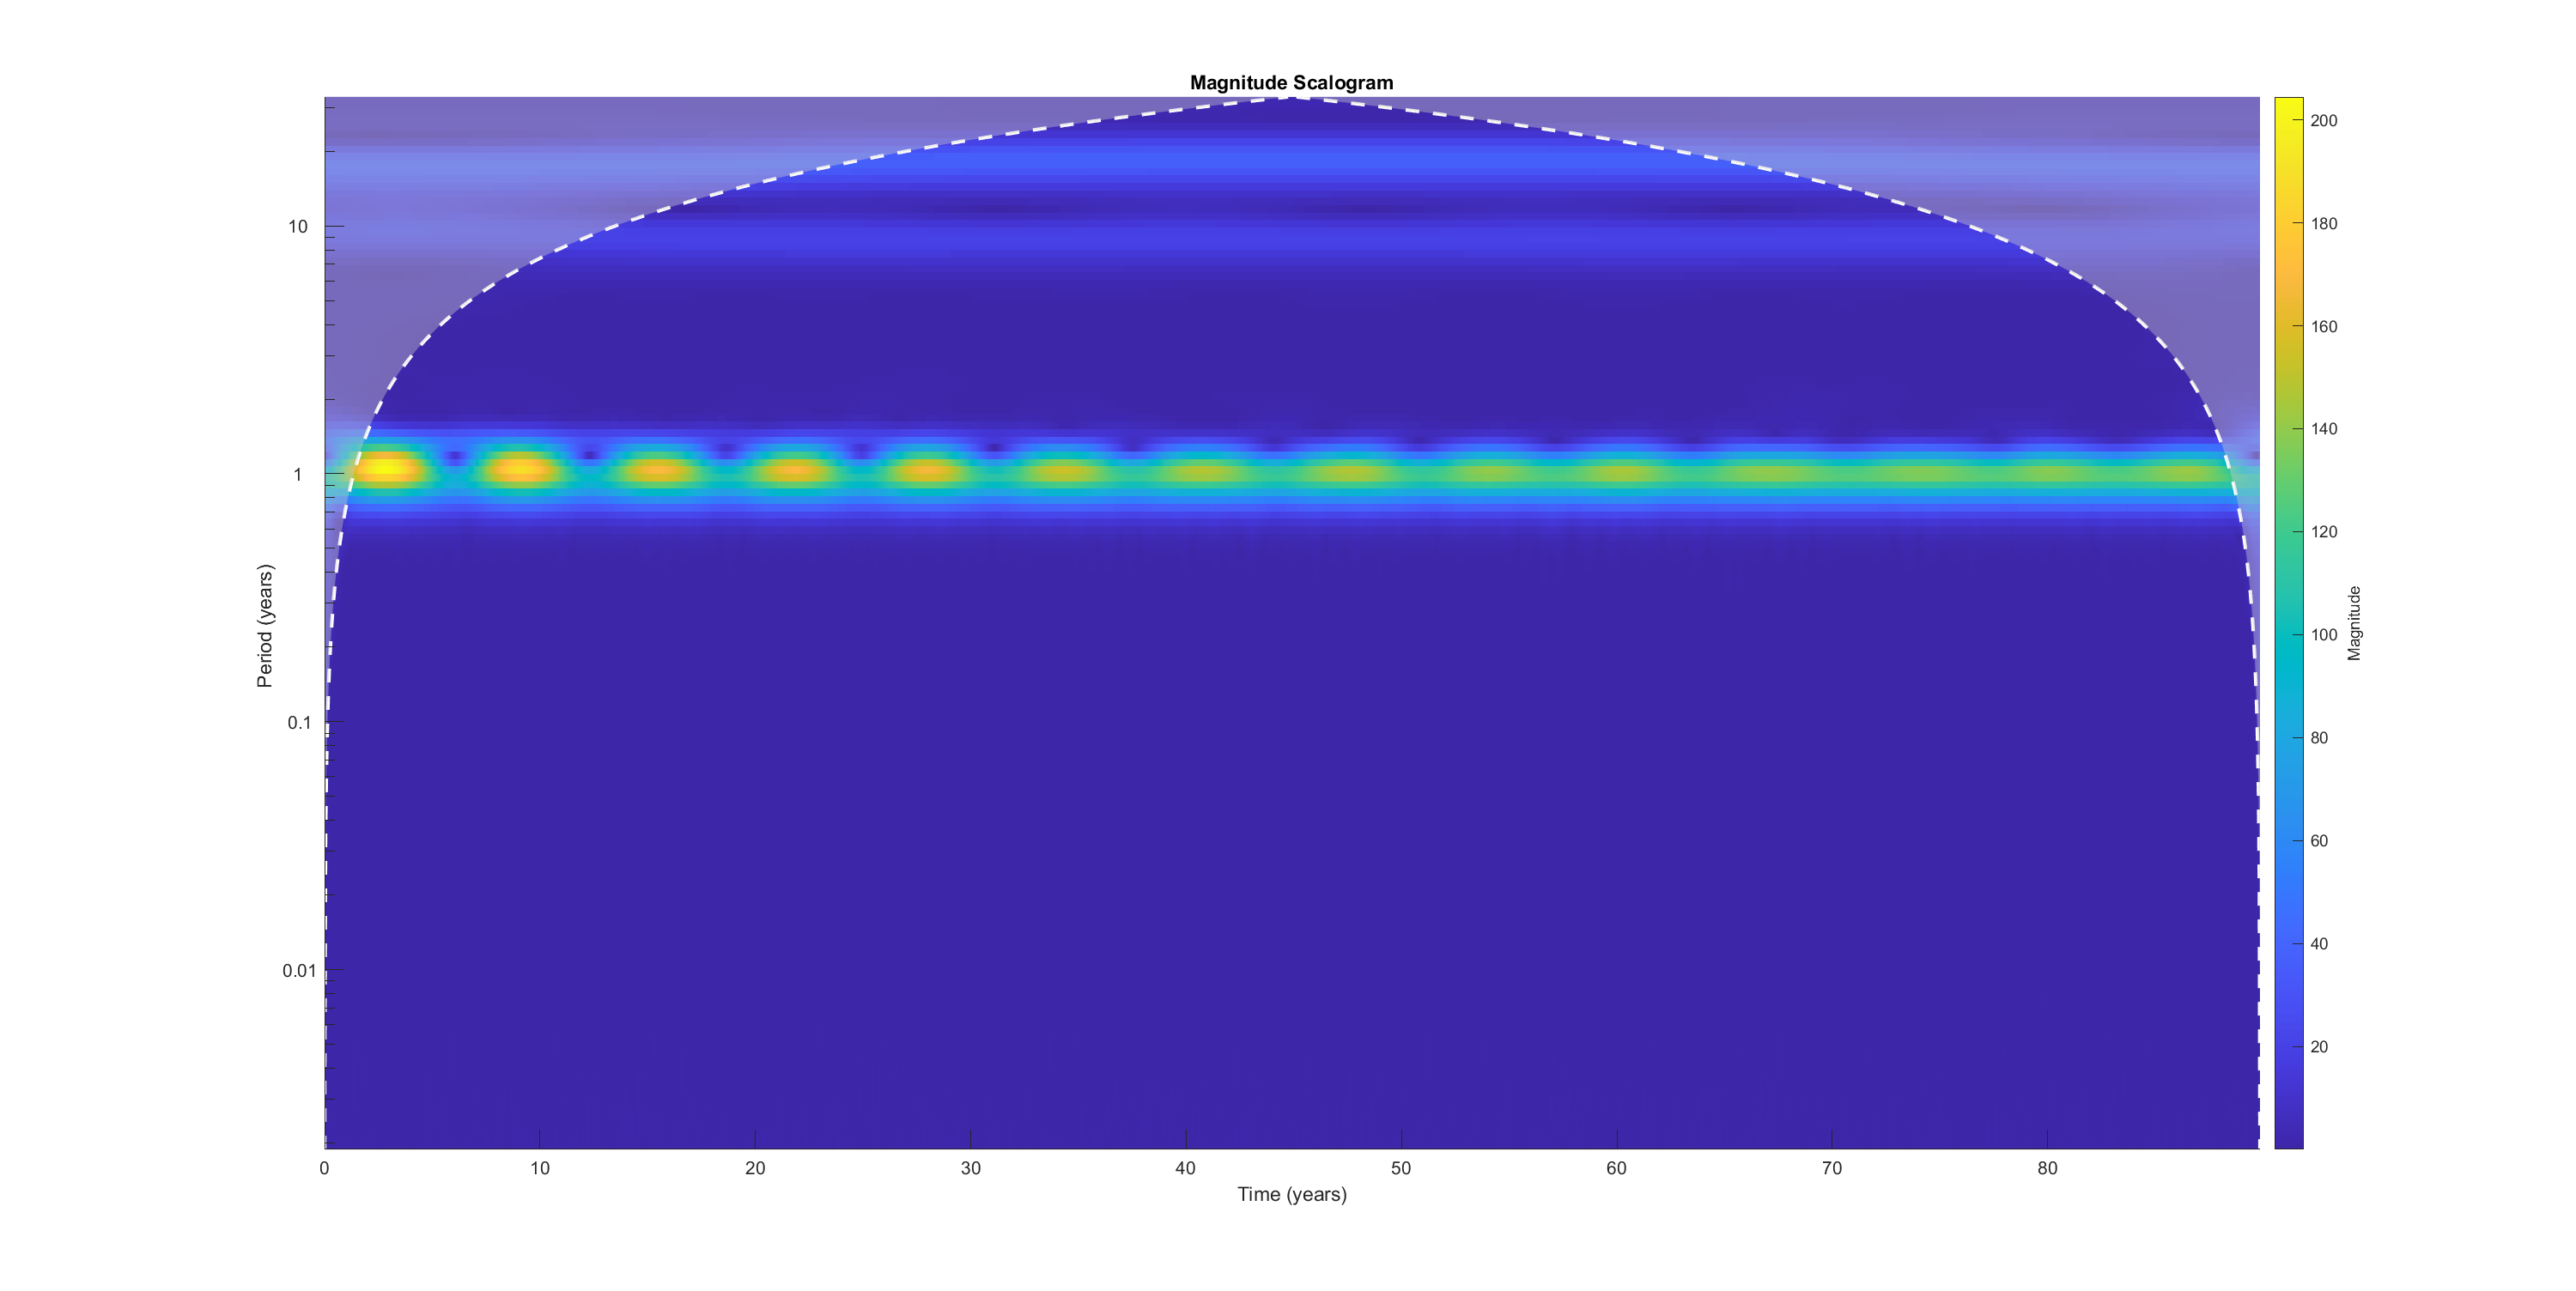
\includegraphics[width=1\linewidth]{inc/task1_cwt2}}
	\caption{Вейвлет-скейлограмма 2}
	\label{task1_cwt2}
\end{figure}

Теперь можно увидеть все гармоники на СПМ и вейвлет-скейлограмме. Следует отметить что появился новый пик на Чандлеровской частоте после ЛР6 и усилилась годовая гармоника на положительной полуоси.

\newpage
Попробуем использовать функцию ChandPantFreqFilter(), но сначала закомментируем строчку с применением фильтра Пантелеева (рис. \ref{task4}):

\begin{figure}[!h]
	\center{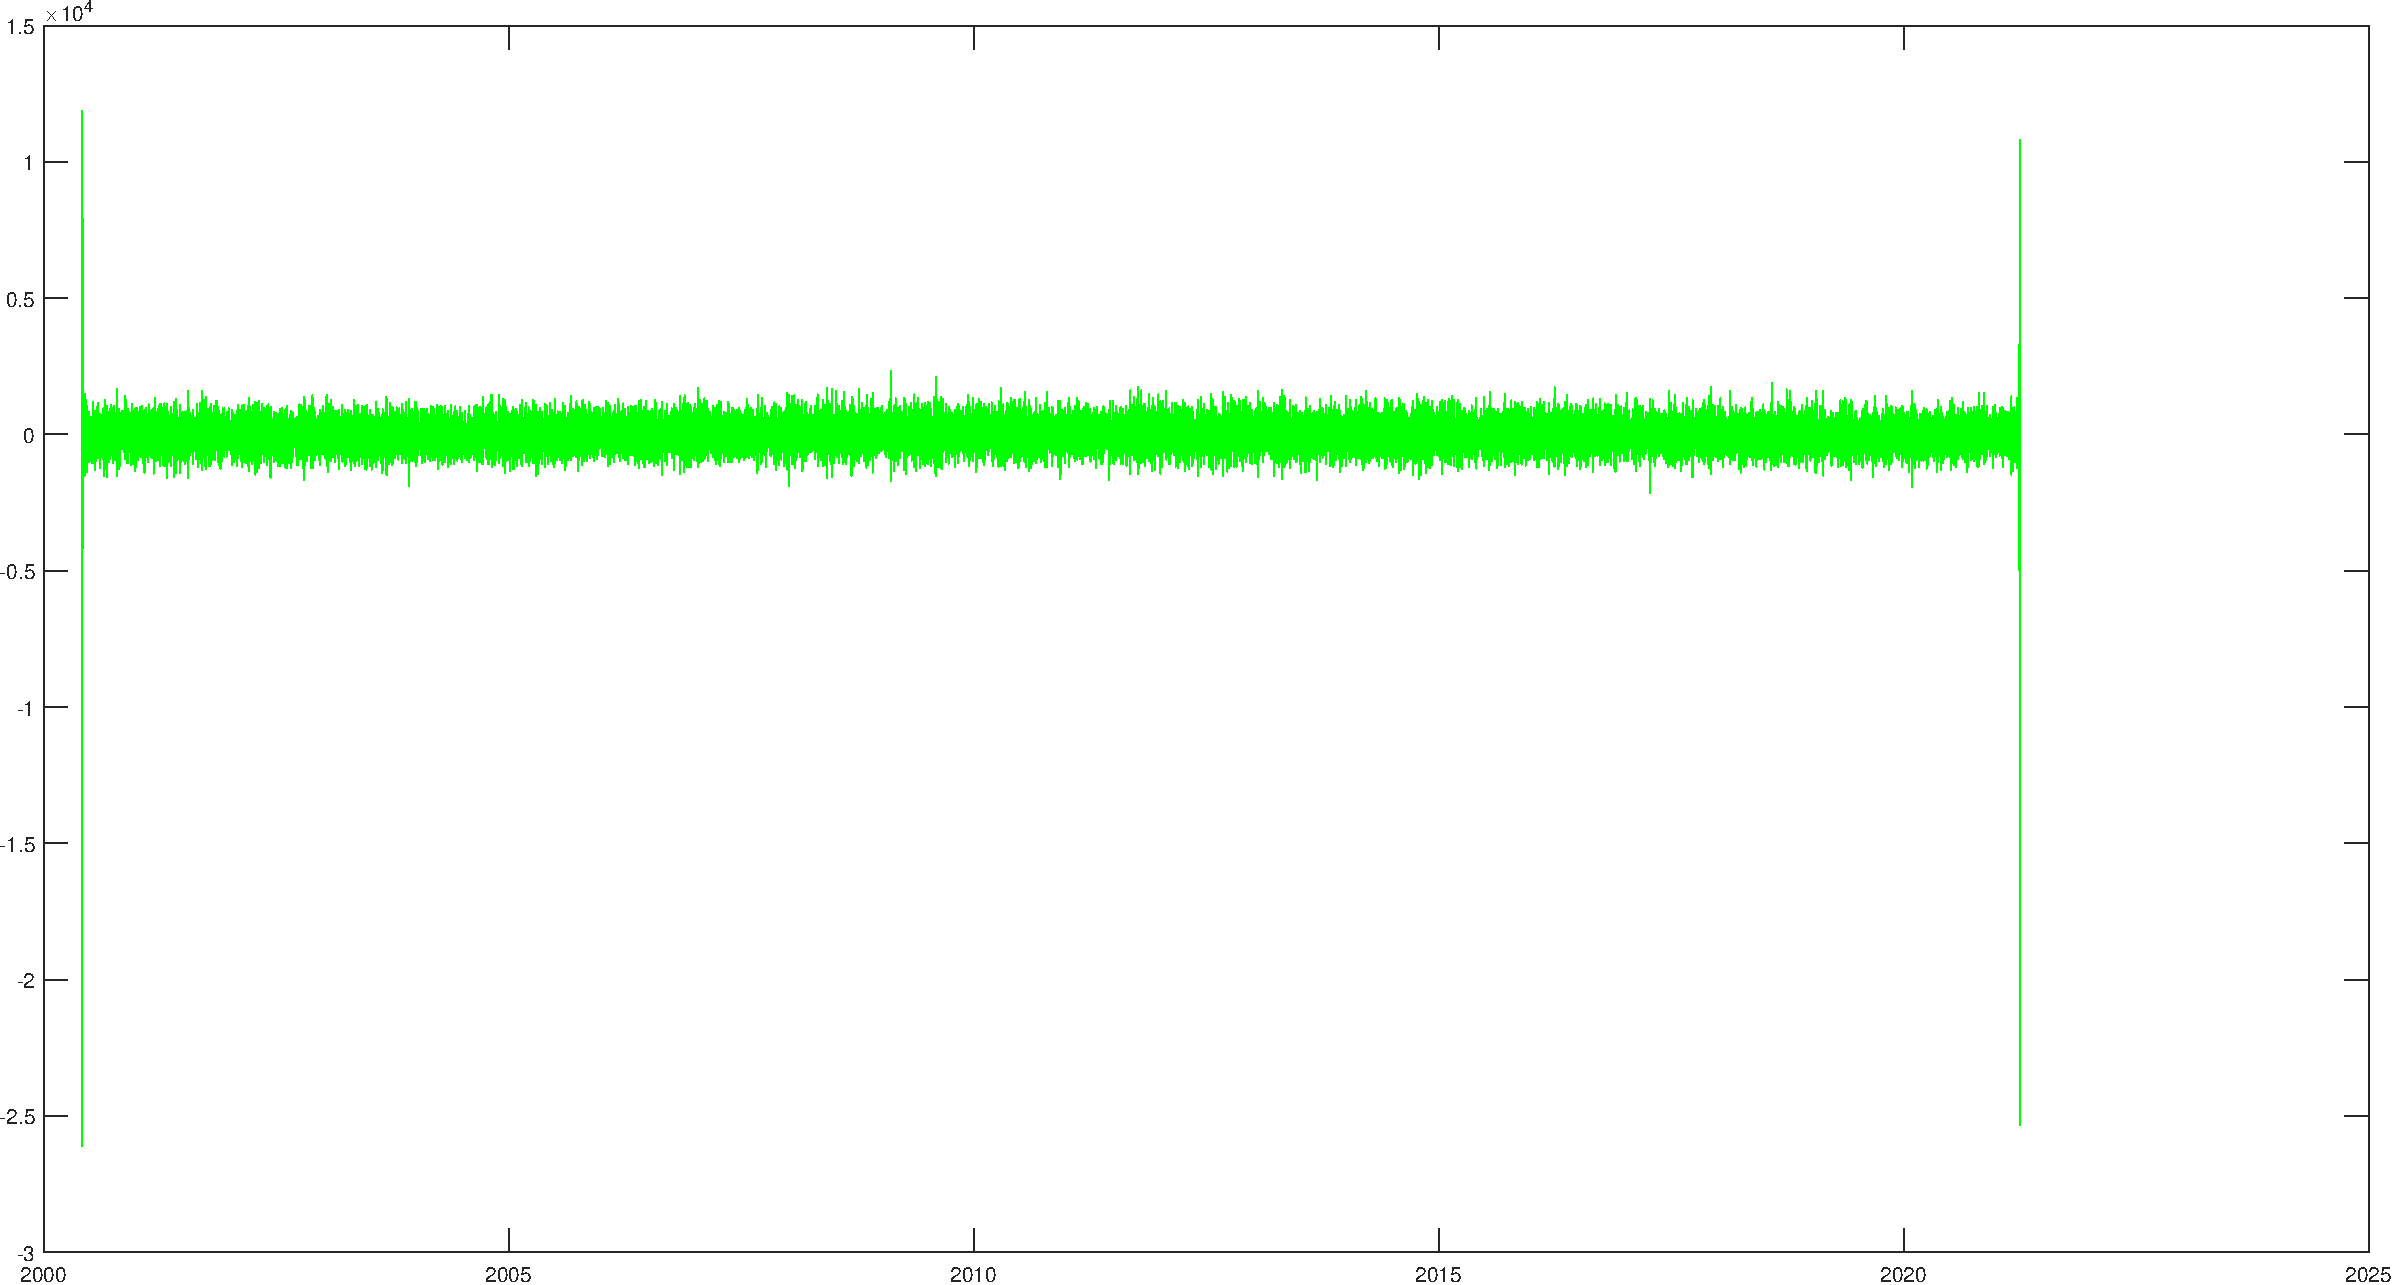
\includegraphics[width=1\linewidth]{inc/task4}}
	\caption{Результат ChandPantFreqFilter() без фильтра Пантелеева}
	\label{task4}
\end{figure}

Как видно по графику \ref{task4} получившийся сигнал не похож на входной сигнал из ЛР6 даже из-за малейших шумов, поэтому вернем применение фильтра Пантелеева в функцию ChandPantFreqFilter() (рис. \ref{task5}):

\begin{figure}[!h]
	\center{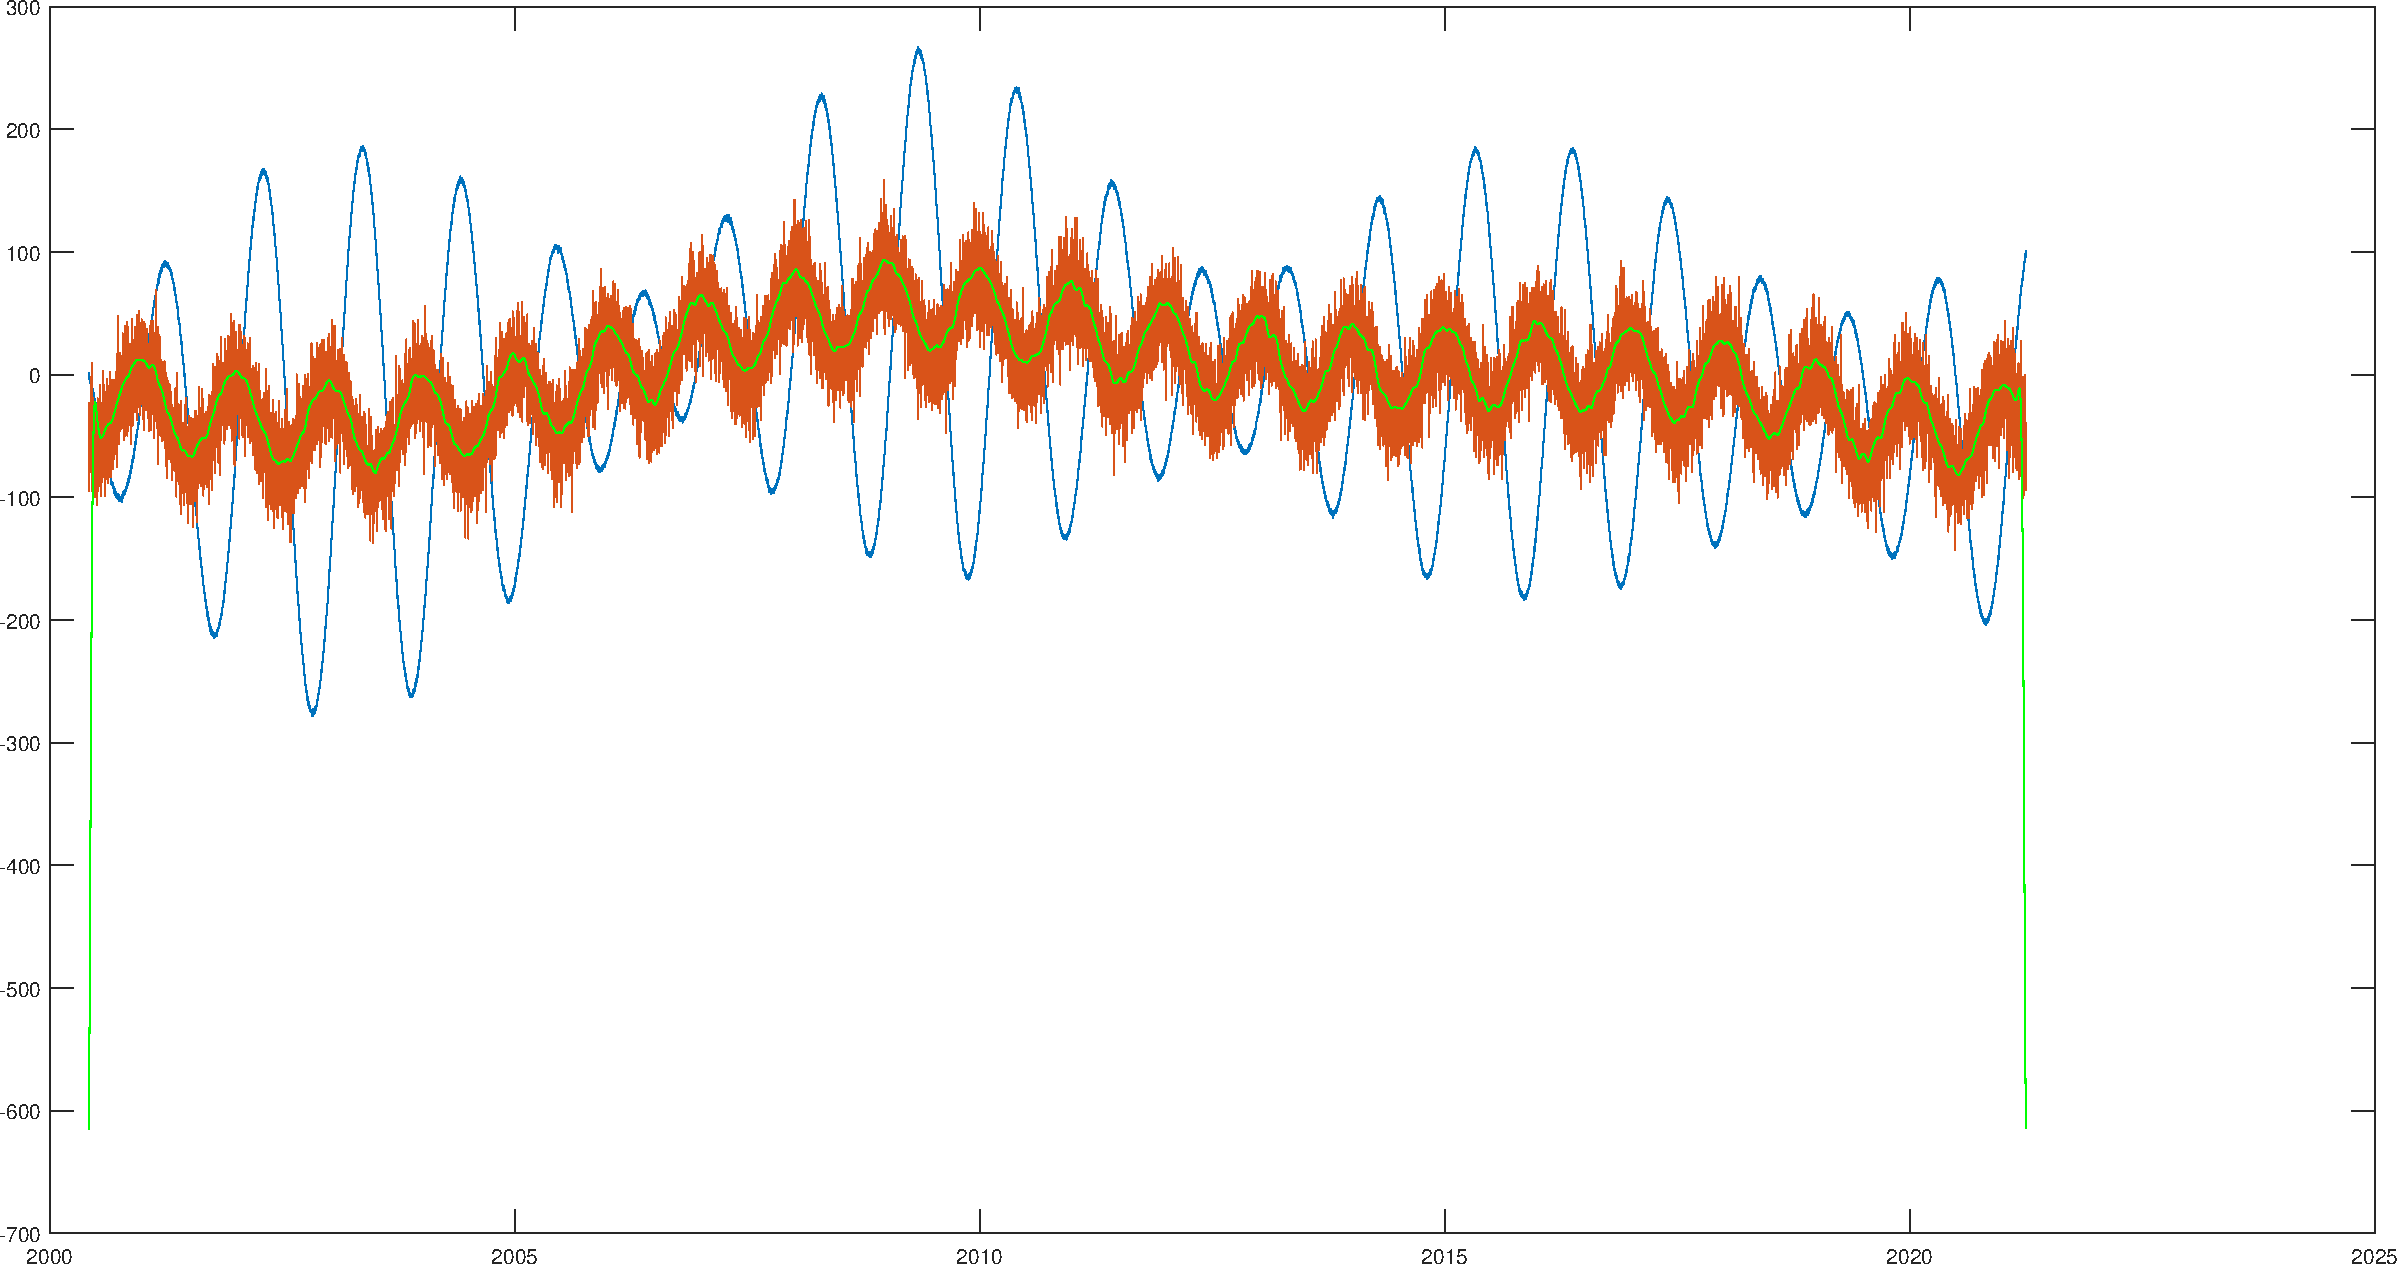
\includegraphics[width=1\linewidth]{inc/task5}}
	\caption{Результат ChandPantFreqFilter() с фильтром Пантелеева}
	\label{task5}
\end{figure}

\newpage
Вот теперь получилось восстановить входной сигнал из ЛР6, но, очевидно, уловить все колебания изначального авторегрессионного шума невозможно.

Также посмотрим на СПМ отфильтрованного сигнала (синим) в сравнении с исходным (оранжевым), чтобы убедится в правильности полученного результата (рис. \ref{task5_spectr}):

\begin{figure}[!h]
	\center{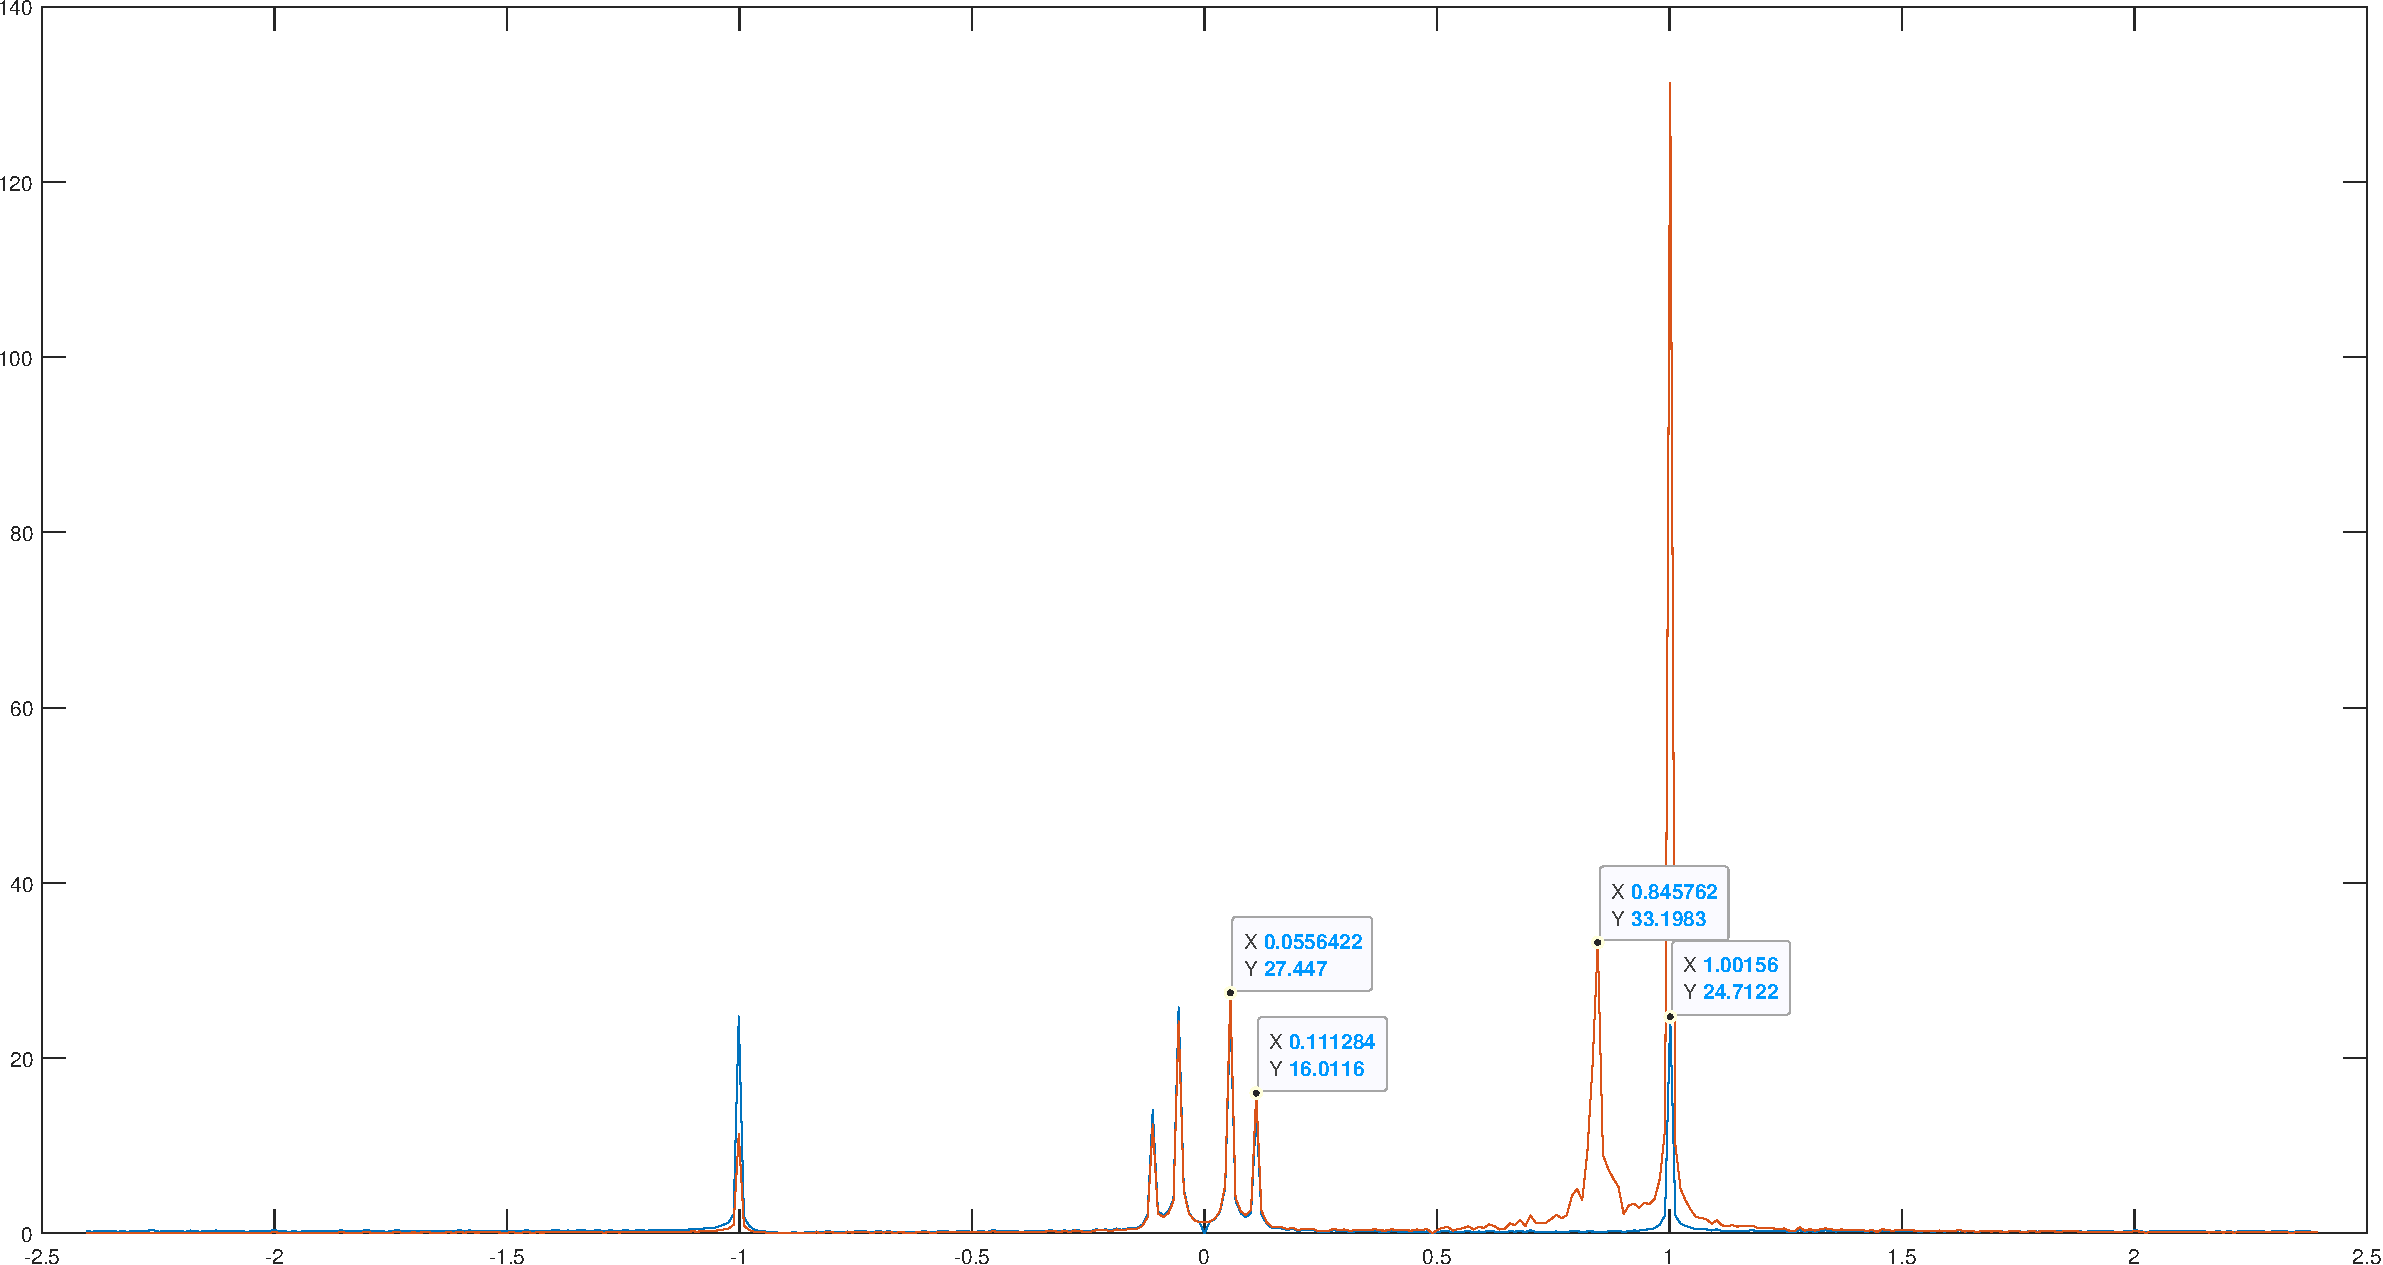
\includegraphics[width=1\linewidth]{inc/task5_spectr}}
	\caption{СПМ отфильтрованного и изначального сигналов}
	\label{task5_spectr}
\end{figure}

\end{document}